\documentclass[10pt]{article}
\usepackage{icmlko}

\icmlmeta{IP 파운데이션 월드모델}{199}{순환을 없앴더니 신호가 없어졌다}{노트 198이 ``격차와 $k$ 를 같은 구간에서 재는 순환''을 지목했다. 토막을 셋으로 잘라 없앴다 --- 안쪽이 유보를 따라오는데, 그사이 재는 대상 자체가 바뀌어 버렸다}

\begin{document}

\twocolumn[
\icmlheader

\begin{abstract}
노트 198에서 축소 비율 $k$ 의 안쪽 곡선과 유보 곡선의 상관이 $+$0.036 으로
사실상 0 이었고, 그 까닭을 ``격차를 안쪽 평가 구간에서 재고 $k$ 도 같은
구간에서 고르는 순환''으로 읽었다. 없앴다 --- 학습 구간을 셋으로 잘라
1토막으로 적합하고 2토막에서 격차를 재고, 1$+$2토막으로 적합해 3토막에서
$k$ 를 고른다. \textbf{진단은 옳았다} --- 안쪽 $\leftrightarrow$ 유보 상관이
$+$0.036 에서 \textbf{$+$0.893} 이 된다. 안쪽이 유보를 거의 그대로
따라간다. \textbf{그런데 유보 곡선 자체가 뒤집혔다.} 노트 198에서는 $k$ 를
키울수록 $+$0.3852 $\to$ $+$0.3998 로 올랐는데, 여기서는 $+$0.3852 $\to$
\textbf{$+$0.3560} 으로 내려간다. 재는 대상이 바뀐 것이다 ---
\textbf{격차 추정이 시끄러워졌다.} 토막이 셋이 되면 각 도메인의 격차를
2토막(전체 학습의 25\%)에서 재게 되고, \textbf{웹툰의 부호가 $-$0.016 에서
$+$0.017 로 뒤집힌다.} 웹툰이 혼자로 가면 유보 $\rho$ 가 $+$0.248 에서
$+$0.090 으로 떨어지고 판 기여가 $-$0.044 다 --- 그 하나가 높은 $k$ 를
무너뜨린다. 애니도 뒤집힌다($+$0.003 $\to$ $-$0.019). \textbf{규약이 또
막았다} --- 봉우리 0.072 · 단조 0.786 으로 문턱 0.8 에 아슬아슬하게 못
미친다. 통과했으면 $k{=}2$ 를 골라 $+$0.3852 로 이분($+$0.3955)보다
$-$0.010 이었을 것이다. \textbf{다섯 번째로 옳게 막았다.} 결론은 맞바꿈이다:
\textbf{순환을 없애는 것과 격차를 정확히 재는 것이 같은 자료를 놓고
다툰다.} 토막을 늘리면 안쪽이 유보를 따라가지만 따라갈 대상이 망가진다.
\textbf{채택은 노트 197의 이분 규칙 그대로다}($+$0.3955).
\end{abstract}
]

\begin{figure*}[t]
\centering
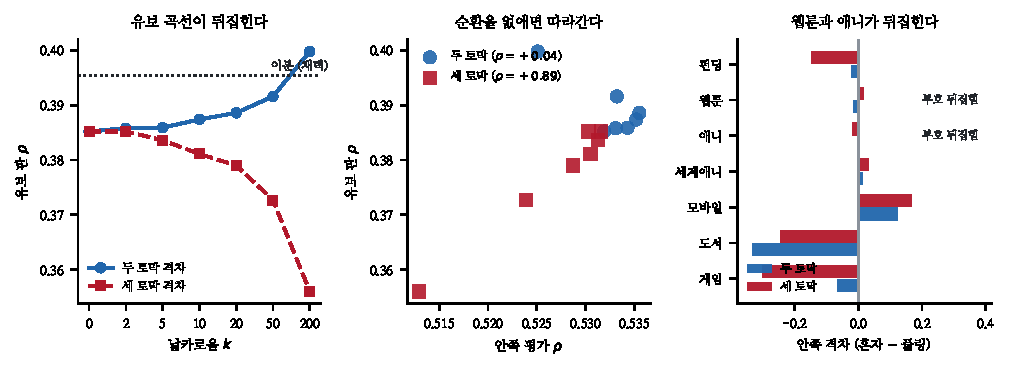
\includegraphics[width=\textwidth]{figs/loop.pdf}
\caption{왼쪽 --- 유보 곡선이 뒤집힌다. 가운데 --- 순환을 없애면 따라간다.
오른쪽 --- 웹툰과 애니가 뒤집힌다.}
\end{figure*}

\section{진단은 옳았다}

\begin{table}[t]
\centering\tsize
\caption{안쪽 $\leftrightarrow$ 유보 상관.}
\begin{tabular}{lr}
\toprule
두 토막 (노트 198 · 순환 있음) & $+$0.036 \\
\textbf{세 토막 (순환 없음)} & \textbf{$+$0.893} \\
\bottomrule
\end{tabular}
\end{table}

\claimx{\textbf{순환을 없애니 안쪽이 유보를 따라간다.} 노트 198의 읽기가
맞았다 --- 같은 자료로 격차를 재고 $k$ 를 고르면 안쪽 곡선이 유보와 무관해
진다.}{이 흐름에서 ``까닭''이 맞은 것이 오랜만이다 --- 노트 186 · 195 ·
198 에서 세 번 연속 틀렸다.}

\section{그런데 대상이 바뀌었다}

\begin{table}[t]
\centering\tsize
\caption{$k$ 를 키울 때 유보 판 $\rho$.}
\begin{tabular}{rrr}
\toprule
$k$ & 두 토막 격차 & 세 토막 격차 \\
\midrule
0 & .3852 & .3852 \\
20 & .3886 & .3790 \\
\textbf{200} & \textbf{.3998} & \textbf{.3560} \\
\bottomrule
\end{tabular}
\end{table}

\begin{table}[t]
\centering\tsize
\caption{안쪽 격차. 부호가 둘 뒤집힌다.}
\begin{tabular}{lrrl}
\toprule
& 두 토막 & 세 토막 & \\
\midrule
모바일 & $+$.123 & $+$.168 & \\
세계애니 & $+$.014 & $+$.032 & \\
\textbf{웹툰} & \textbf{$-$.016} & \textbf{$+$.017} & \textbf{뒤집힘} \\
\textbf{애니} & \textbf{$+$.003} & \textbf{$-$.019} & \textbf{뒤집힘} \\
펀딩 & $-$.021 & $-$.146 & \\
게임 & $-$.064 & $-$.302 & \\
도서 & $-$.332 & $-$.244 & \\
\bottomrule
\end{tabular}
\end{table}

\claimx{\textbf{웹툰의 부호가 뒤집히고 그 하나가 다 무너뜨린다.} 웹툰이
혼자로 가면 유보 $\rho$ 가 $+$0.248 에서 $+$0.090 으로 떨어지고 판 기여가
$-$0.044 다 --- 높은 $k$ 에서 잃는 $-$0.044 가 그 곡선의 전부다.}{노트
198이 ``잡음이 크기에 있고 신호가 부호에 있다''고 적었는데, 토막을 늘리니
\textbf{부호에도 잡음이 들어왔다.}}

\claimx{\textbf{맞바꿈이다.} 순환을 없애려면 격차와 $k$ 를 다른 토막에서
재야 하고, 그러면 격차를 재는 토막이 전체 학습의 25\%로 줄어 부호가
흔들린다.}{같은 자료를 놓고 두 요구가 다툰다 --- \textbf{노트 191이 잰
``학습행 대 평가행'' 맞바꿈과 같은 모양이고, 이번엔 세 갈래다.}}

\section{다섯 번째로 옳게 막았다}

\claimx{\textbf{규약이 막았다} --- 봉우리 0.072 · 단조 0.786. 문턱 0.8 에
0.014 못 미친다.}{통과했으면 $k{=}2$ 를 골라 $+$0.3852 였을 것이다 ---
이분($+$0.3955)보다 $-$0.010. \textbf{아슬아슬하게 옳았고, 문턱은 노트
194에서 다른 자료로 정한 값이다.}}

\begin{table}[t]
\centering\tsize
\caption{규약이 막은 다섯.}
\begin{tabular}{lrl}
\toprule
& 막았으면 & \\
\midrule
노트 190 챔피언 조정 & $-$.0104 & 옳음 \\
노트 193 앞으로-사슬 & $-$.0110 & 옳음 \\
노트 193 세 번 평균 & --- & 옳음 \\
노트 198 축소 비율 & $-$.0069 & 옳음 \\
\textbf{노트 199 순환 없앤 축소} & \textbf{$-$.0103} & \textbf{옳음} \\
\bottomrule
\end{tabular}
\end{table}

\claimx{\textbf{다섯 번 다 옳았다.} 봉우리 · 단조 지수는 노트 190 · 194 에서
각각 네 점 · 다섯 점으로 문턱을 그은 것인데 그 뒤 다섯 번을 독립으로
맞혔다.}{반대편도 적어 둔다 --- 노트 195 · 198 에서 보이지 않는 이득
$+$0.007 · $+$0.004 를 놓쳤다. \textbf{계산서는 막은 쪽이 $-$0.039, 놓친
쪽이 $+$0.011 이다.}}

\begin{table}[t]
\centering\tsize
\caption{이 갈래(노트 197$\sim$199)의 최종.}
\begin{tabular}{lr}
\toprule
완전 분리 & .3445 \\
완전 풀링 & .3822 \\
축소 비율 (두 토막 · 막힘) & .3886 \\
축소 비율 (세 토막 · 막힘) & .3852 \\
\textbf{이분 (노트 197 · 채택)} & \textbf{.3955} \\
\bottomrule
\end{tabular}
\end{table}

\begin{table}[t]
\centering\tsize
\caption{남은 것.}
\begin{tabular}{ll}
\toprule
\textbf{격차} & 부호만 쓰되 더 많은 자료로 재려면 \\
문턱 0.8 & 이번에 0.014 차로 갈렸다 \\
\textbf{다음 갈래} & 이 갈래는 능형만 --- 트리로 \\
\bottomrule
\end{tabular}
\end{table}

첫 줄에 아직 안 해 본 길이 하나 있다. 격차의 \emph{부호}만 필요하다면 그것을
재는 데 전체 학습을 다 쓸 수 있다 --- 도메인마다 접힘 교차로 ``혼자 대
풀링''을 재면 25\%가 아니라 100\%를 쓴다. 순환은 접힘이 막는다.
\textbf{그러면 부호가 안 흔들리고 $k$ 도 고를 수 있다.} 다만 접힘은 시간을
섞으므로 노트 182가 잰 시들기에 낙관적이 된다 --- \textbf{시간 접힘으로
하면 다시 토막이 작아진다.} 빠져나갈 곳이 있는지가 이 갈래에 남은 마지막
질문이다.

\end{document}
